%%%%%%%%%%%%%%%%%%%%%%%%%%%%%%%%%%%%%%%%%
% Beamer Presentation
% LaTeX Template
% Version 1.0 (10/11/12)
%
% This template has been downloaded from:
% http://www.LaTeXTemplates.com
%
% License:
% CC BY-NC-SA 3.0 (http://creativecommons.org/licenses/by-nc-sa/3.0/)
%
%%%%%%%%%%%%%%%%%%%%%%%%%%%%%%%%%%%%%%%%%

%----------------------------------------------------------------------------------------
%	PACKAGES AND THEMES
%----------------------------------------------------------------------------------------

\documentclass{beamer}

\mode<presentation> {
	
	% The Beamer class comes with a number of default slide themes
	% which change the colors and layouts of slides. Below this is a list
	% of all the themes, uncomment each in turn to see what they look like.
	
	%\usetheme{default}
	%\usetheme{AnnArbor}
	%\usetheme{Antibes}
	%\usetheme{Bergen}
	%\usetheme{Berkeley}
	%\usetheme{Berlin}
	%\usetheme{Boadilla}
	%\usetheme{CambridgeUS}
	%\usetheme{Copenhagen}
	%\usetheme{Darmstadt}
	%\usetheme{Dresden}
	%\usetheme{Frankfurt}
	%\usetheme{Goettingen}
	%\usetheme{Hannover}
	%\usetheme{Ilmenau}
	%\usetheme{JuanLesPins}
	%\usetheme{Luebeck}
	\usetheme{Madrid}
	%\usetheme{Malmoe}
	%\usetheme{Marburg}
	%\usetheme{Montpellier}
	%\usetheme{PaloAlto}
	%\usetheme{Pittsburgh}
	%\usetheme{Rochester}
	%\usetheme{Singapore}
	%\usetheme{Szeged}
	%\usetheme{Warsaw}
	
	% As well as themes, the Beamer class has a number of color themes
	% for any slide theme. Uncomment each of these in turn to see how it
	% changes the colors of your current slide theme.
	
	%\usecolortheme{albatross}
	%\usecolortheme{beaver}
	%\usecolortheme{beetle}
	%\usecolortheme{crane}
	%\usecolortheme{dolphin}
	%\usecolortheme{dove}
	%\usecolortheme{fly}
	%\usecolortheme{lily}
	%\usecolortheme{orchid}
	%\usecolortheme{rose}
	%\usecolortheme{seagull}
	%\usecolortheme{seahorse}
	%\usecolortheme{whale}
	%\usecolortheme{wolverine}
	
	%\setbeamertemplate{footline} % To remove the footer line in all slides uncomment this line
	%\setbeamertemplate{footline}[page number] % To replace the footer line in all slides with a simple slide count uncomment this line
	
	%\setbeamertemplate{navigation symbols}{} % To remove the navigation symbols from the bottom of all slides uncomment this line
}

\usepackage{graphicx} % Allows including images
\usepackage{booktabs} % Allows the use of \toprule, \midrule and \bottomrule in tables
\usepackage{epigraph}
\usepackage{animate}

%----------------------------------------------------------------------------------------
%	TITLE PAGE
%----------------------------------------------------------------------------------------

\title[Intro to probability]{An introduction to probability} % The short title appears at the bottom of every slide, the full title is only on the title page

\author{Ben Lambert} % Your name
\institute[Univ. of Oxford] % Your institution as it will appear on the bottom of every slide, may be shorthand to save space
{
	University of Oxford \\ % Your institution for the title page
	\medskip
	\textit{ben.c.lambert@gmail.com} % Your email address
}
\date{\today} % Date, can be changed to a custom date

\begin{document}
	
	\begin{frame}
		\titlepage % Print the title page as the first slide
	\end{frame}

	\begin{frame}
		\frametitle{Who am I?}
		
		\begin{itemize}
			\item Statistician working mainly in epidemiology.
			\item Claim to probability fame: born in the same town where Thomas Bayes lived (Tunbridge Wells, UK).
		\end{itemize}
		
		\begin{figure}[ht]
			\centerline{\includegraphics[width=0.6\textwidth]{./figures/tunbridgeWells.jpg}}
		\end{figure}
		
	\end{frame}

	\begin{frame}
		\frametitle{Course outline}
		
		\begin{itemize}
			\item 9am-10.30am: follow along lecture and problems
			\item 10.30am-10.45am: refreshments break
			\item 10.45am-midday: follow along lecture and problems
		\end{itemize}
		
		\vspace{0.5cm}
		
		Note: problems will involve both pen and paper type questions \textit{and} those using R.
		
		Levels: each problem set will have at least one \textit{advanced} question.
		
		Time: if you don't finish the questions in time, don't worry. There are answers to these here: \url{https://github.com/ben18785/introduction_to_probability}.
		
	\end{frame}

	\begin{frame}
		\frametitle{Resources}
		
		\begin{itemize}
			\item Introduction to probability, Blitzstein and Hwang. Open source book available here: \url{https://projects.iq.harvard.edu/stat110/home}
			\item Seeing theory, Kunin et al. A beautiful online resource that has lots of creative ways to think about probability. \url{https://seeing-theory.brown.edu/}
		\end{itemize}
		
	\end{frame}

	\begin{frame}
		\frametitle{Outline}
		\tableofcontents
	\end{frame}

	\section{What is probability and why do we need it?}
	\frame{\tableofcontents[currentsection]}
	
	\begin{frame}
		\frametitle{What is probability?}
		\epigraph{Mathematics is the logic of certainty; probability [theory] is the [mathematical] logic of uncertainty}{Bitzstein and Hwang, 2019}
		
	\end{frame}

	\begin{frame}
		\frametitle{Why do we need probability theory?}
		
		Life and science are full of unknown things. We say these things are \textit{uncertain}.
		
		Faced with these, we can give up; \textit{Probability theory} gives us a way to make assumptions about uncertain phenomena which allows us to make progress with understanding without having to know everything.
		
		\epigraph{There are known knowns. These are things we know that we know. There are known unknowns. That is to say, there are things that we know we don't know. But there are also unknown unknowns. There are things we don't know we don't know.}{Donald Rumsfeld, 2002}
		
	\end{frame}
	
	\begin{frame}
		\frametitle{Who uses probability?}
		It is used in:
		
		\begin{itemize}
			\item Statistics: probability is the foundational language of it
			\item Biology: e.g. inheritance of genes
			\item Meteorology: e.g. weather forecasts are generated using probabilities
			\item Epidemiology: e.g. analysing randomised clinical trials and fitting models to epidemiological data
			\item Physics: our current best explanation of the universe at small scales (quantum theory) is based on probability
		\end{itemize}
		
		
	\end{frame}

	\begin{frame}
		\frametitle{The difficulties of probability}
		
		If we rely on our intuitions, we can easily get things wrong when dealing with uncertainty.
		
		\vspace{0.5cm}
		
		 So, we need careful mathematical analysis.
		 
		 \vspace{0.5cm}
		
		Fortunately, \textit{simulation} using R / Python / etc. can also really help us to understand.
		
	\end{frame}

	\section{Probability and counting}
	\frame{\tableofcontents[currentsection]}
	
	\begin{frame}
		\frametitle{Blitzstein and Hwang's Pebble World}
		
		As an example, consider reaching into a bag to pull out one of nine pebbles: we call this \textit{pebble world}.
		
		\begin{figure}[ht]
			\centerline{\includegraphics[width=0.6\textwidth]{./figures/pebble_world_base.png}}
		\end{figure}
		
	\end{frame}


	\begin{frame}
		\frametitle{Outcomes}
		
		An \textit{outcome} is a possible result of some activity. Here pulling one particular pebble out of the bag would be an outcome.
		
		\begin{figure}[ht]
			\centerline{\includegraphics[width=0.6\textwidth]{./figures/pebble_world_single.png}}
		\end{figure}
		
	\end{frame}

	\begin{frame}
		\frametitle{Sample spaces}
		
		The \textit{sample space}, $S$, is the \textit{set} of all possible outcomes of an experiment. Here, it is the set of all pebbles.
		
		\begin{figure}[ht]
			\centerline{\includegraphics[width=0.6\textwidth]{./figures/pebble_world_sample_space.png}}
		\end{figure}
		
	\end{frame}

	\begin{frame}
		\frametitle{Events}
		
		An \textit{event} is a \textit{set} of possible outcomes. For example, below event $A$ corresponds to selecting one of five pebbles; event $B$ to selecting one of two.
		
		As we can see, two or more events can happen at once.
		
		\begin{figure}[ht]
			\centerline{\includegraphics[width=0.6\textwidth]{./figures/pebble_world.png}}
		\end{figure}
		
	\end{frame}


	\begin{frame}
		\frametitle{Probabilities of events}
		
		What do we mean by the probability of $A$ occurring? We write this as: $\mathbb{P}(A)$.
		
		\begin{figure}[ht]
			\centerline{\includegraphics[width=0.6\textwidth]{./figures/pebble_world_proba.png}}
		\end{figure}
		
	\end{frame}

	\begin{frame}
		\frametitle{Probabilities from counting}
		
		If all pebbles equally likely to be drawn:
		
		 \begin{equation}
		 	\mathbb{P}(A) = \frac{\text{number of pebbles in } A}{\text{number of pebbles in } S} = \frac{5}{9}
		 \end{equation}
	 
	 \begin{figure}[ht]
	 	\centerline{\includegraphics[width=0.6\textwidth]{./figures/pebble_world_proba.png}}
	 \end{figure}
		
	\end{frame}

	\begin{frame}
		\frametitle{Probability of an event in $S$}
		
		Consider the probability that some event in $S$ occurs:
		
		\begin{equation}
			\mathbb{P}(S) = \frac{\text{number of pebbles in } S}{\text{number of pebbles in } S} = \frac{9}{9} = 1
		\end{equation}
		
		\begin{figure}[ht]
			\centerline{\includegraphics[width=0.6\textwidth]{./figures/pebble_world_probs.png}}
		\end{figure}
		
	\end{frame}

	\begin{frame}
		\frametitle{Probability of null event}
		What about the probability that no event in $S$ occurs?
		
		\begin{equation}
			\mathbb{P}(\text{not }S) = \frac{0}{9} = 0
		\end{equation}
		
		\begin{figure}[ht]
			\centerline{\includegraphics[width=0.6\textwidth]{./figures/pebble_world_probnots.png}}
		\end{figure}
		
	\end{frame}

	\begin{frame}
		\frametitle{Defining probability}
		
		A probability of an event must be bounded between 0 and 1\footnote{Note: ``impossible'' isn't 100\% accurate here but you can start out by thinking of probabilities this way.}.
		
		\begin{figure}[ht]
			\centerline{\includegraphics[width=0.8\textwidth]{./figures/probability.png}}
		\end{figure}
		
	\end{frame}

	\begin{frame}
		\frametitle{Interpreting probabilities}
		
		There are many schools of thought for what probabilities mean. Two common ones are:
		
		\begin{itemize}
			\item \textit{Frequentist}. Think of probabilities as frequencies that would be obtained under many (actually infinite) repetitions of an experiment. E.g. flipping a coin a large number of times and using fraction of heads as $\mathbb{P}(H)$.
			\item \textit{Bayesian}. Suppose probabilities reflect an underlying subjective belief about the chance of events occurring.
		\end{itemize}
		
	\end{frame}

		\begin{frame}
		\frametitle{An event not occurring}
		We can also determine the probability that $A$ does not occur:
		
		\begin{equation}
			\mathbb{P}(\text{not } A) = \frac{\text{number of pebbles not in } A}{\text{number of pebbles in } S} = \frac{4}{9}
		\end{equation}
		
		\begin{figure}[ht]
			\centerline{\includegraphics[width=0.6\textwidth]{./figures/pebble_world_probnota.png}}
		\end{figure}
		
	\end{frame}

	\begin{frame}
		\frametitle{Question}
		
		\Large Can anyone think of an alternative way of determining the probability that $A$ does not occur?
		
	\end{frame}

	\begin{frame}
		\frametitle{Question}
		
		\Large Can anyone think of an alternative way of determining the probability that $A$ does not occur?
		
		\begin{equation}
			\mathbb{P}(\text{not } A) = \mathbb{P}(S) - \mathbb{P}(A) = 1 - \mathbb{P}(A) = 1 - \frac{5}{9}
		\end{equation}
		
	\end{frame}

	\begin{frame}
		\frametitle{Combinations of events: intersection}
		
		We can determine the probability of $A$ \textit{and} $B$ occurring by determining the overlap between these two events:
		
		\begin{equation}
			\mathbb{P}(A \cap  B) = \mathbb{P}(A, B) = \frac{\text{number of pebbles in both } A \text{ and } B}{\text{number of pebbles in } S} = \frac{1}{9}
		\end{equation}
		
		\begin{figure}[ht]
			\centerline{\includegraphics[width=0.6\textwidth]{./figures/pebble_world_and.png}}
		\end{figure}
		
	\end{frame}

	\begin{frame}
		\frametitle{Combinations of events: union}
		
		We can determine the probability of $A$ \textit{and/or} $B$ occurring by:
		
		\begin{equation}
			\mathbb{P}(A \cup B) = \frac{\text{number of pebbles in either } A \text{ or } B \text{ or both}}{\text{number of pebbles in } S} = \frac{6}{9}
		\end{equation}
	
	\begin{figure}[ht]
		\centerline{\includegraphics[width=0.6\textwidth]{./figures/pebble_world_or.png}}
	\end{figure}
		
	\end{frame}

	\begin{frame}
		\frametitle{Question}
		
		\Large Can anyone think of an alternative way of determining the probability of the union of $A$ and $B$?
		
	\end{frame}

	\begin{frame}
		\frametitle{Question}
		
		\Large Can anyone think of an alternative way of determining the probability of the union of $A$ and $B$?
		
		\begin{align}
			\mathbb{P}(A \cup B) &= \mathbb{P}(A) + \mathbb{P}(B) - \mathbb{P}(A \cap B)\\
			&= \frac{5}{9} + \frac{2}{9} - \frac{1}{9} = \frac{6}{9}
		\end{align}
		
		
	\end{frame}
	
	
	\begin{frame}
		\Large Questions?
	\end{frame}
	
	
	\begin{frame}
		\frametitle{Problems: dice}
		
		\begin{figure}[ht]
			\centerline{\includegraphics[width=0.2\textwidth]{./figures/dice.png}}
		\end{figure}
	
	Consider a fair six-sided die with numbers 1-6 on each face that is thrown once.
		
		\begin{enumerate}
			\item What's the probability that a six is thrown?
			\item What's the probability that an even number is thrown?
			\item Suppose two dice are thrown, what's the probability that the their sum adds up to 11 or less?
			\item \textit{Advanced}: if six dice are thrown, what's the probability that one of each of the numbers is obtained? If you like, use R to check your result.
		\end{enumerate}
		
	\end{frame}


	\begin{frame}
		\frametitle{Example: a random sweet}
		
		Suppose you visit a sweet shop. The shop produces both ice cream and cake. It also offers three sauces: strawberry, vanilla and chocolate.
		
		\vspace{0.5cm}
		
		Unlike most shops, you don't get a choice. The way the shopkeeper allocates food is they randomly choose either a ice cream or cake (selecting either with equal probability). They then randomly select a sauce from the three available (again with equal probability of each).
		
		\vspace{0.5cm}
		
		Suppose you like anything with chocolate sauce. What's the probability that you obtain this?
		
	\end{frame}

	\begin{frame}
		\frametitle{A naive way to count}
		
		How many outcomes are there? Cake with strawberry, cake with vanilla, cake with chocolate, ice cream with strawberry, ice cream with vanilla, ice cream with chocolate.  So there are \textit{six} outcomes.
		
		\vspace{0.5cm}
		
		How many of these have chocolate sauce: two.
		
		\vspace{0.5cm}
		
		\begin{equation}
			\mathbb{P}(\text{chocolate}) = \frac{2}{6}
		\end{equation}
		
	\end{frame}


	\begin{frame}
		\frametitle{A sweet tree: making counting easier}
		
		\begin{figure}[ht]
			\centerline{\includegraphics[width=0.7\textwidth]{./figures/tree.pdf}}
		\end{figure}
		
	\end{frame}

	\begin{frame}
		\frametitle{Using trees to determine probabilities}
		
		\begin{figure}[ht]
			\centerline{\includegraphics[width=0.7\textwidth]{./figures/tree-prob.pdf}}
		\end{figure}
		
	\end{frame}

	\begin{frame}
		\frametitle{What's the probability of cake with chocolate sauce?}
		
		\begin{figure}[ht]
			\centerline{\includegraphics[width=0.4\textwidth]{./figures/tree-prob-choc-cake.pdf}}
		\end{figure}
	
	To obtain this probability, we take the probabilities obtained along the path and multiply:
	
	\begin{equation}
		\mathbb{P}(\text{chocolate cake}) = \frac{1}{2} \times \frac{1}{3} = \frac{1}{6}
	\end{equation}


	This is equivalent to counting possibilities (if all choices equally likely).
	
	\end{frame}

	\begin{frame}
		\frametitle{Chocolate probability}
		
		\begin{figure}[ht]
			\centerline{\includegraphics[width=0.4\textwidth]{./figures/tree-prob-choc.pdf}}
		\end{figure}
	
	Sum up probabilities:
	
	\begin{equation}
		\mathbb{P}(\text{chocolate}) = \frac{1}{2} \times \frac{1}{3} +  \frac{1}{2} \times \frac{1}{3} = \frac{2}{6}
	\end{equation}
	
	\end{frame}

	\begin{frame}
		\frametitle{A particular shopkeeper}
		Now suppose we visit another shop. Here, the shopkeeper allocates cake or ice cream as before (i.e. with equal probability). The differ in terms of how they offer sauces:
		
		\vspace{0.5cm}
		
		If a cake is chosen, they randomly select sauces: vanilla with probability $1/2$, chocolate with probability $1/3$ and strawberry with probability $1/6$.
		
		\vspace{0.5cm}
		
		If an ice cream is chosen, they randomly select sauces: vanilla with probability $1/6$, chocolate with probability $1/2$ and strawberry with probability $1/3$.
		
		\vspace{0.5cm}
		
		Now what is the probability an item with chocolate sauce is obtained?
		
	\end{frame}

	\begin{frame}
		\frametitle{The problem with counting}
		
		Now different outcomes have different weights, so can't use counting. But tree still works.
		
		\begin{figure}[ht]
			\centerline{\includegraphics[width=0.4\textwidth]{./figures/tree-prob-choc-2.pdf}}
		\end{figure}
		
		Sum up probabilities:
		
		\begin{equation}
			\mathbb{P}(\text{chocolate}) = \frac{1}{2} \times \frac{1}{3} +  \frac{1}{2} \times \frac{1}{2} = \frac{5}{12}
		\end{equation}
		
	\end{frame}


	\section{Conditional probability}
	\frame{\tableofcontents[currentsection]}
	
	\begin{frame}
		\frametitle{What is conditioning?}
		
		When we receive new information, we want to take it into account to make better predictions.
		
		\vspace{0.5cm}
		
		Effectively, learning something about the world (typically) helps us to reduce our own uncertainty.
		
		\vspace{0.5cm}
		
		\textit{Conditioning} is how this is handled in statistics.
		
	\end{frame}


	\begin{frame}
		\frametitle{Back to pebble world}
		
		\begin{figure}[ht]
			\centerline{\includegraphics[width=0.5\textwidth]{./figures/pebble_world_and.png}}
		\end{figure}
		
		If we know that $A$ has occurred, what's the probability that $B$ has occurred? We write this \textit{conditional} probability as:
		
		\begin{equation}
			\mathbb{P}(B|A)
		\end{equation}
	
		which reads, ``The probability that $B$ occurs given that $A$ has.''
		
	\end{frame}

	\begin{frame}
		\frametitle{Shrinking sample space}
		
		If we know $A$ has occurred, our sample space shrinks.
		
		\begin{figure}[ht]
			\centerline{\includegraphics[width=0.5\textwidth]{./figures/pebble_world_conditional.pdf}}
		\end{figure}
	
		So now we can just count:
		
		\begin{equation}
			\mathbb{P}(B|A) = \frac{1}{5}
		\end{equation}
		
	\end{frame}

	\begin{frame}
		\frametitle{Law of conditional probability}
		
		The below rule effectively renormalises the sample space to calculate updated probabilities:
		
		\begin{equation}
			\mathbb{P}(B|A) = \frac{\mathbb{P}(A \cap B)}{\mathbb{P}(A)}
		\end{equation}
	
		In our example:
		
		\begin{equation}
			\mathbb{P}(B|A) = \frac{1/9}{5/9} = \frac{1}{5}
		\end{equation}
		
	\end{frame}


	\begin{frame}
		\frametitle{Question}
		
		Is $\mathbb{P}(A|B)$ equal to $\mathbb{P}(B|A)$?
		
	\end{frame}

	\begin{frame}
		\frametitle{Inverse conditional}
		
		No due to different shrunk sample spaces.
			
		\begin{equation}
			\mathbb{P}(A|B) = \frac{\mathbb{P}(A \cap B)}{\mathbb{P}(B)} = \frac{1/9}{2/9} = \frac{1}{2}
		\end{equation}
			
		\begin{figure}[ht]
			\centerline{\includegraphics[width=0.5\textwidth]{./figures/pebble_world_conditional1.pdf}}
		\end{figure}
			
	\end{frame}

	\begin{frame}
		\frametitle{Trees and conditional probability: back to the shop}
		
		\begin{figure}[ht]
			\centerline{\includegraphics[width=0.4\textwidth]{./figures/tree-prob-1.pdf}}
		\end{figure}
	
	Question: What's the probability that we get given strawberry sauce given that we receive a cake?
		
	\end{frame}

	\begin{frame}
		\frametitle{Shrunk sample space}
		
		\begin{figure}[ht]
			\centerline{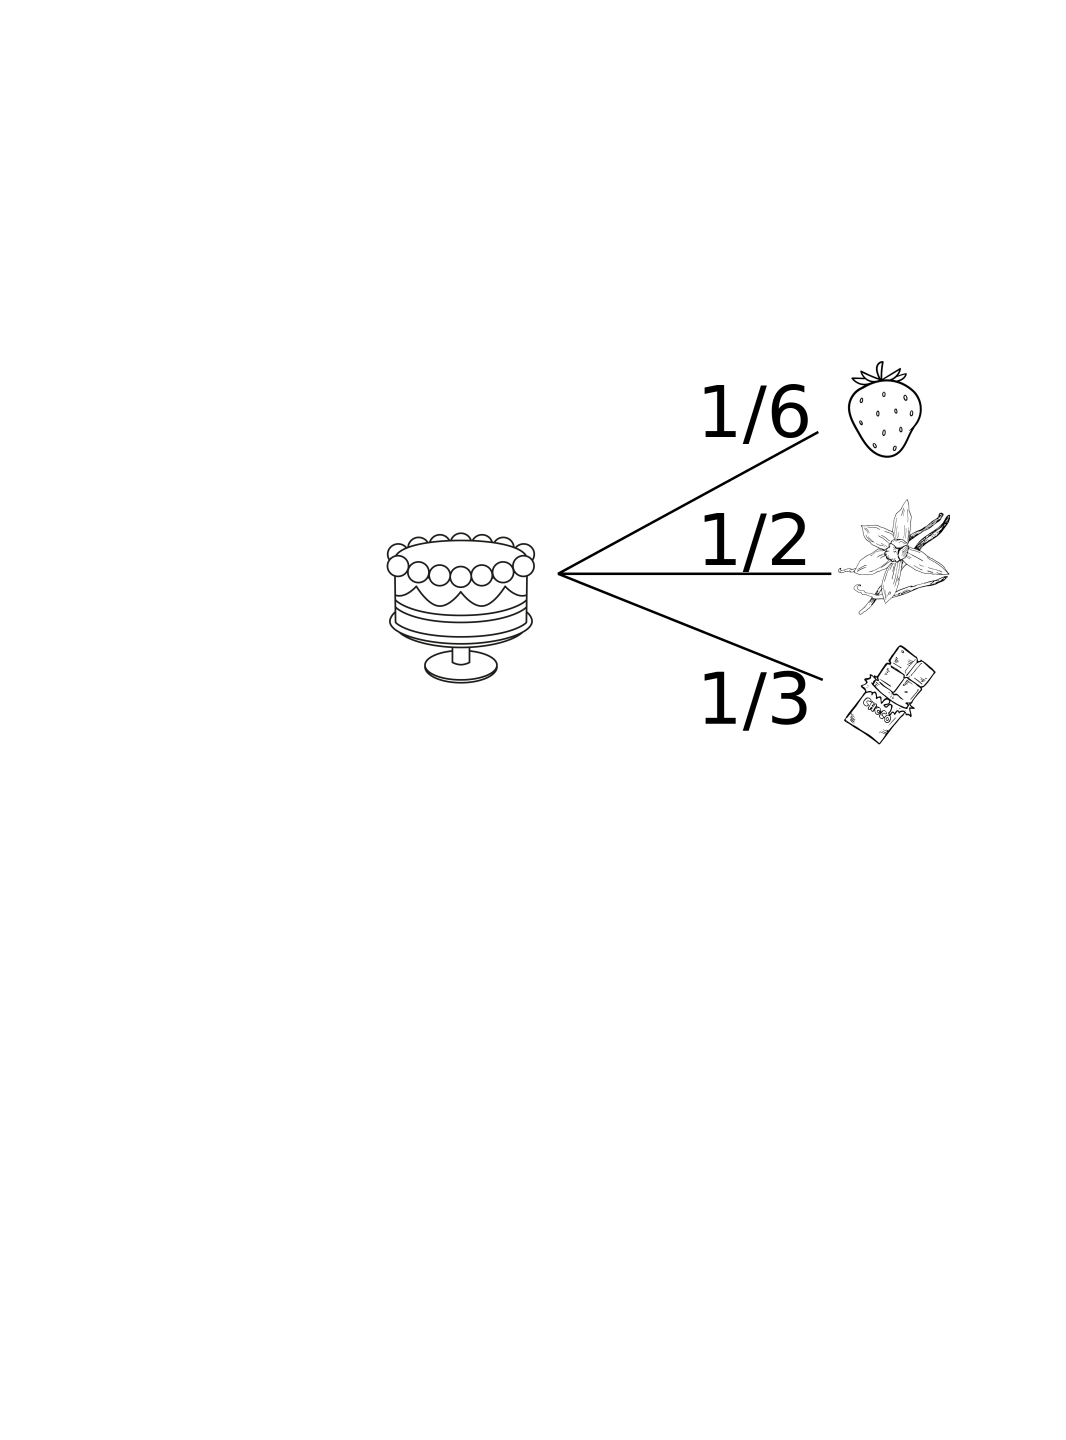
\includegraphics[width=0.4\textwidth]{./figures/tree-prob-1-shrunk.pdf}}
		\end{figure}
	
	So, we simply read off $1/6$.
		
	\end{frame}

	\begin{frame}
		\frametitle{Question}
		
		What's the probability that we received an ice-cream given that we got vanilla sauce?
		
		
	\end{frame}

	\begin{frame}
		\frametitle{Why is this not correct?}
		

		\begin{figure}[ht]
			\centerline{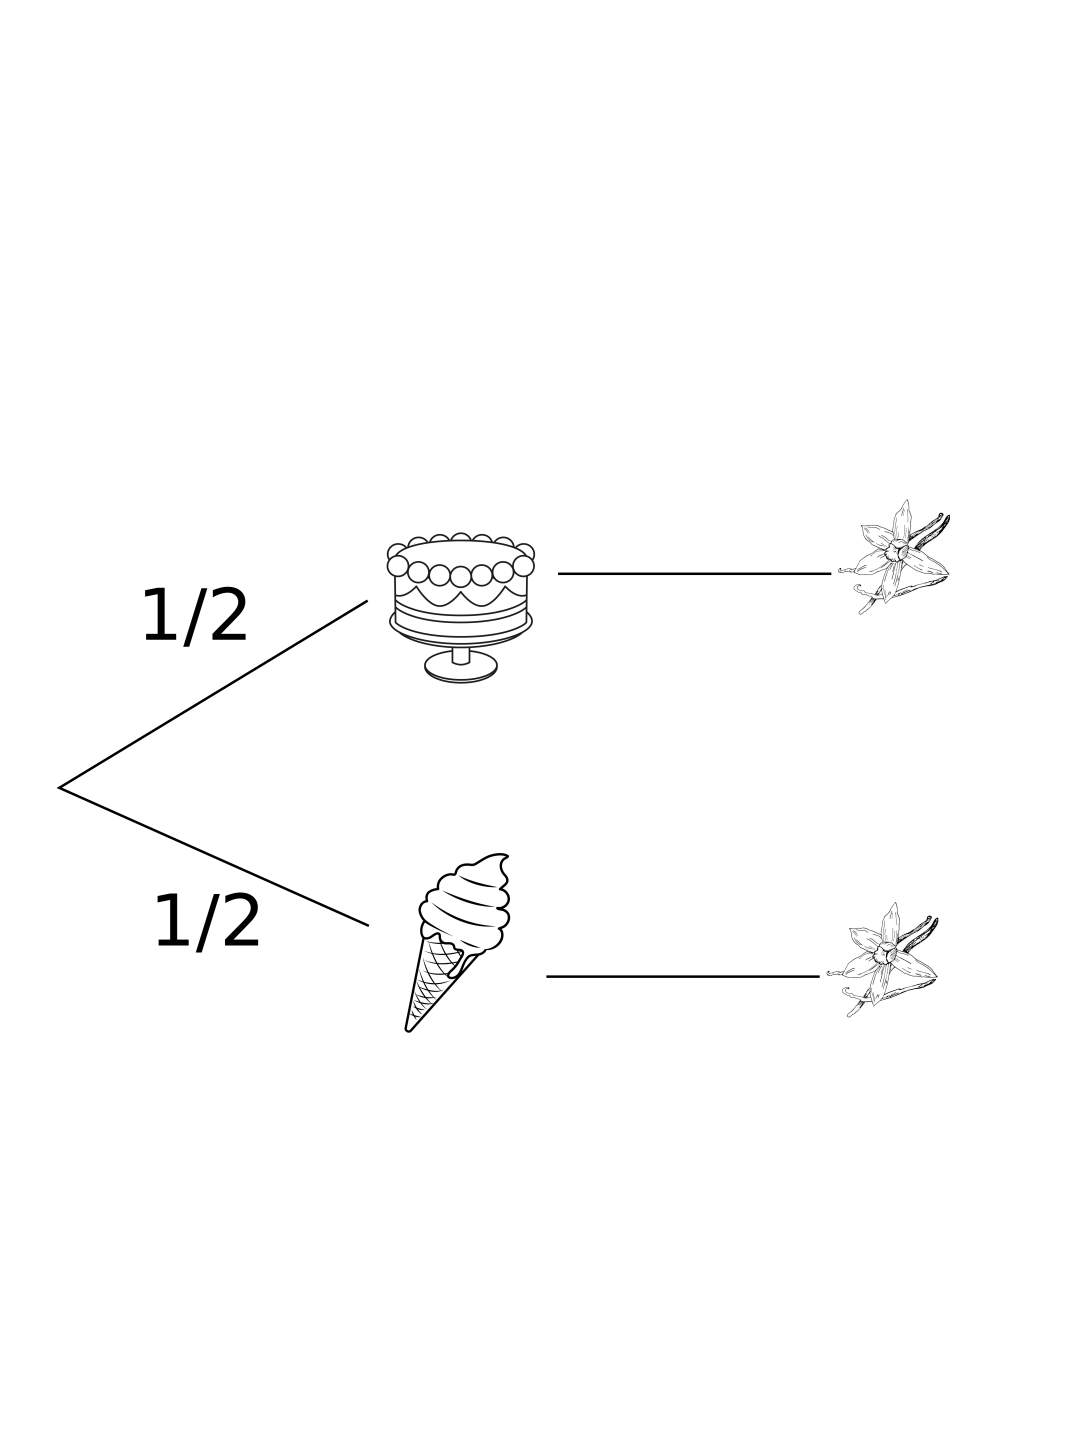
\includegraphics[width=0.6\textwidth]{./figures/tree-prob-2.pdf}}
		\end{figure}
	
	Meaning that:
	
	\begin{equation}
		\mathbb{P}(\text{ice cream}|\text{vanilla}) = \frac{1}{2}
	\end{equation}
	
	\end{frame}


	\begin{frame}
		\frametitle{Apply law of conditional probability}
		
		\begin{equation}
			\mathbb{P}(\text{ice cream}|\text{vanilla}) = \frac{\mathbb{P}(\text{ice cream} \cap \text{vanilla})}{\mathbb{P}(\text{vanilla})} = \frac{1/2 \times 1/6}{\mathbb{P}(\text{vanilla})}
		\end{equation}
	
	Question: how to calculate the denominator $\mathbb{P}(\text{vanilla})$?
		
	\end{frame}

	\begin{frame}
		\frametitle{Vanilla overall}
		
		\begin{figure}[ht]
			\centerline{\includegraphics[width=0.3\textwidth]{./figures/tree-prob-1-vanilla.pdf}}
		\end{figure}

	\begin{equation}
		\mathbb{P}(\text{vanilla}) = \frac{1}{2} \times \frac{1}{2} + \frac{1}{2} \times \frac{1}{6} = \frac{1}{3}
	\end{equation}

	Meaning:

		\begin{equation}
			\mathbb{P}(\text{ice cream}|\text{vanilla}) = \frac{1/2 \times 1/6}{\mathbb{P}(\text{vanilla})} = \frac{1/12}{1/3} = \frac{1}{4}
		\end{equation}
	
	\end{frame}

	\begin{frame}
		\frametitle{Independence}
	
	We say that events $A$ and $B$ are \textit{independent} if:
	
	\begin{equation}
		\mathbb{P}(A|B) =  \mathbb{P}(A)
	\end{equation}

	in other words, knowing that $B$ has occurred gives us no additional information about whether $A$ has occurred.
		
	\end{frame}

	\begin{frame}
		\frametitle{Are $A$ and $B$ independent?}
		
			\begin{figure}[ht]
			\centerline{\includegraphics[width=0.6\textwidth]{./figures/pebble_world_prob_independent.pdf}}
		\end{figure}
		
	\end{frame}

	\begin{frame}
		\frametitle{Are $A$ and $B$ independent?}
		
		\begin{figure}[ht]
			\centerline{\includegraphics[width=0.3\textwidth]{./figures/pebble_world_prob_independent.pdf}}
		\end{figure}
	
	Yes!
	
	\begin{equation}
		\mathbb{P}(A) =  \frac{3}{9} = \frac{1}{3}
	\end{equation}

	and:
	
	\begin{equation}
		\mathbb{P}(A|B) =  \frac{1}{3}
	\end{equation}

	So $\mathbb{P}(A|B) = \mathbb{P}(A)$.
		
	\end{frame}
	
	
	\begin{frame}
		\frametitle{Redux: Are $A$ and $B$ independent?}
		
		\begin{figure}[ht]
			\centerline{\includegraphics[width=0.6\textwidth]{./figures/pebble_world_prob_disjoint.pdf}}
		\end{figure}
		
	\end{frame}

		\begin{frame}
		\frametitle{Redux: Are $A$ and $B$ independent?}
		
		\begin{figure}[ht]
			\centerline{\includegraphics[width=0.3\textwidth]{./figures/pebble_world_prob_disjoint.pdf}}
		\end{figure}
	
	No. Knowing that $B$ occurs tells me that $A$ could not have occurred:
	
	\begin{equation}
		\mathbb{P}(A) =  \frac{1}{3}
	\end{equation}

	and:
	
	\begin{equation}
		\mathbb{P}(A|B) =  0
	\end{equation}

	Events $A$ and $B$ are known as \textit{disjoint}.
		
	\end{frame}

	\begin{frame}
		\frametitle{The law of total probability}
		
		How to determine $\mathbb{P}(A)$?
		
		\begin{figure}[ht]
			\centerline{\includegraphics[width=0.6\textwidth]{./figures/pebble_world_prob_total.pdf}}
		\end{figure}
		
	\end{frame}

	\begin{frame}
		\frametitle{The law of total probability}
		
		\begin{figure}[ht]
			\centerline{\includegraphics[width=0.4\textwidth]{./figures/pebble_world_prob_total.pdf}}
		\end{figure}
		
		\begin{equation}
			\mathbb{P}(A) =  \mathbb{P}(A|B_1)\mathbb{P}(B_1) + \mathbb{P}(A|B_2)\mathbb{P}(B_2) + \mathbb{P}(A|B_3)\mathbb{P}(B_3)
		\end{equation}
	
	More generally (if $B_i$ are disjoint events):
	
	\begin{equation}
		\mathbb{P}(A) =  \sum_{i} \mathbb{P}(A|B_i)\mathbb{P}(B_i)
	\end{equation}
	
	\end{frame}

	\begin{frame}
		\frametitle{Example recap: Law of total probability in action}
		
		\begin{figure}[ht]
			\centerline{\includegraphics[width=0.3\textwidth]{./figures/tree-prob-1-vanilla.pdf}}
		\end{figure}
		
		\begin{equation}
			\mathbb{P}(\text{vanilla}) = \frac{1}{2} \times \frac{1}{2} + \frac{1}{2} \times \frac{1}{6} = \frac{1}{3}
		\end{equation}
	
		Because:
		
		\begin{equation}
			\mathbb{P}(\text{vanilla}) = \mathbb{P}(\text{cake}) \times \mathbb{P}(\text{vanilla}|\text{cake})  +  \mathbb{P}(\text{ice cream}) \times \mathbb{P}(\text{vanilla}|\text{ice cream})
		\end{equation}
	
	\end{frame}

	\begin{frame}
		\Large Questions?
	\end{frame}

		\begin{frame}
		\frametitle{Problems: cards}
		
		Suppose you have a standard deck of 52 cards across four suits -- two of which are red; two black. The cards in order are: 2, 3, 4, 5, 6, 7, 8, 9, 10, J, Q, K, A. Imagine in all cases that cards are drawn from a shuffled deck.
		
		\begin{enumerate}
			\item Consider the event $A$ that a card is a Four and $B$ that the card is black. Are these events $A$ and $B$ independent?
			\item Consider the event $A$ that the card is red and $B$ that it is black. Are these events $A$ and $B$ independent?
			\item What's the probability that, given the card has a value above 8, that it is an Ace?
			\item \textit{Advanced}: suppose two cards are drawn. What's the probability that the second card is an Ace given that the first card is an Ace? What's the probability that second card is an Ace given that at least one is an Ace?
		\end{enumerate}
		
	\end{frame}


	\section{Bayes' rule}
	\frame{\tableofcontents[currentsection]}
	
	\begin{frame}
		\frametitle{Two ways to arrive at same intersection}
		
		\begin{figure}[ht]
			\centerline{\includegraphics[width=0.5\textwidth]{./figures/pebble_world_and.png}}
		\end{figure}
		
		How to calculate $\mathbb{P}(A \cap B)$? Law of conditional probability:
		
		\begin{equation}
			\mathbb{P}(A \cap B) = \mathbb{P}(A) \times \mathbb{P}(B|A) = \mathbb{P}(B) \times \mathbb{P}(A|B)
		\end{equation}
		
	\end{frame}
	
	\begin{frame}
		\frametitle{Bayes' rule}
		
		Combining:
		
		\begin{equation}
		\mathbb{P}(A) \times \mathbb{P}(B|A) = \mathbb{P}(B) \times \mathbb{P}(A|B)
		\end{equation}
		
		which we can rearrange to:
		
		\begin{equation}
		\mathbb{P}(A|B) = \frac{\mathbb{P}(A) \times \mathbb{P}(B|A)}{\mathbb{P}(B)}
		\end{equation}
		
		this is known as \textit{Bayes' rule} and is the foundation of \textit{Bayesian inference}.
		
	\end{frame}
	
	\begin{frame}
		\frametitle{Example use of Bayes' rule: breast cancer screening}
		
		\begin{figure}[ht]
			\includegraphics[width=0.6\textwidth]{./figures/crab2.jpeg}
		\end{figure}
	\end{frame}
	
	\begin{frame}
		\frametitle{Screening probabilities}
		
		
		\begin{figure}[ht]
			\includegraphics[width=0.3\textwidth]{./figures/crab2.jpeg}
		\end{figure}
		
		Suppose:
		\begin{itemize}
			\item The probability that a randomly chosen 40 year old woman has breast cancer is approximately $\frac{1}{100}$.
			\item If a woman has breast cancer the probability they will test positive in a mammography is about 90\%.
			\item However there is a risk of about 8\% of a false positive result of the test.
		\end{itemize}
		
	Question: given that a woman tests positive, what is the probability that she has breast cancer?
		
	\end{frame}
	
	\begin{frame}
		\frametitle{Bayes' rule in action: breast cancer screening}
		
		\textit{Answer:} we want to find the probability the woman has cancer \textit{given} she has tested positive, which we can do via Bayes' rule (it's the same for pmfs as it was for pdfs):
		
		\begin{figure}[ht]
			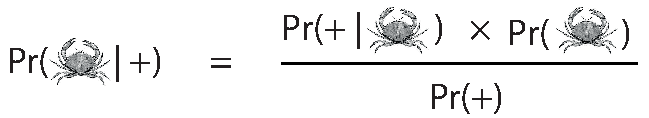
\includegraphics[width=1\textwidth]{./figures/lec1_cancer.pdf}
		\end{figure}
		
	\end{frame}
	
	\begin{frame}
		\frametitle{Bayes' rule in action: breast cancer screening}
		
		\begin{figure}[ht]
			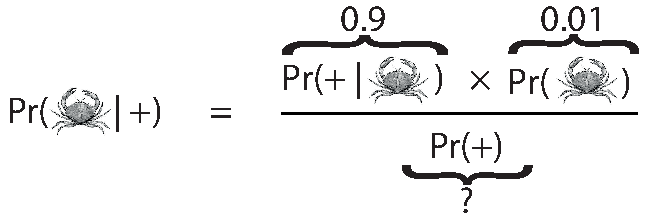
\includegraphics[width=1\textwidth]{./figures/lec1_cancer2.pdf}
		\end{figure}
	
		Calculate denominator using the law of total probability:
		
		\begin{figure}[ht]
			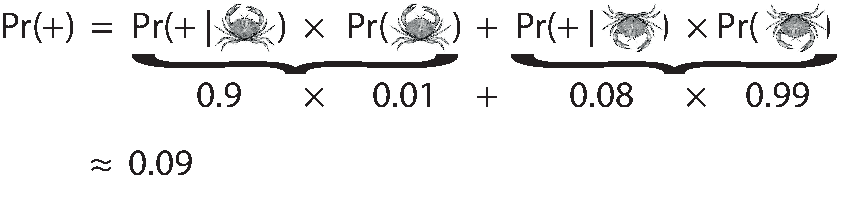
\includegraphics[width=0.8\textwidth]{./figures/lec1_cancer3.pdf}
		\end{figure}
		
	\end{frame}
	
	\begin{frame}
		\frametitle{Bayes' rule in action: breast cancer screening}
		Putting this into Bayes' rule:
		
		\begin{figure}[ht]
			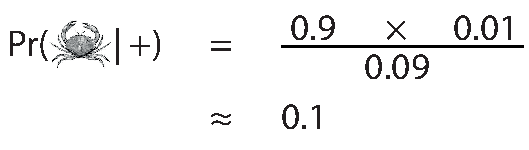
\includegraphics[width=1\textwidth]{./figures/lec1_cancer4.pdf}
		\end{figure}
		
	\end{frame}

	\begin{frame}
		\frametitle{Intuition: false positives dwarf true ones}
		
		\begin{figure}[ht]
			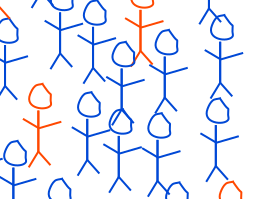
\includegraphics[width=0.7\textwidth]{./figures/breast_cancer_intuition.pdf}
		\end{figure}
		
		
	\end{frame}
	
	\begin{frame}
		\Large Questions?
	\end{frame}
	

	\section{Random variables and probability distributions}
	\frame{\tableofcontents[currentsection]}
	
	\begin{frame}
		\frametitle{Events and random variables}
		Up until now, we have used \textit{events} to describe outcomes.
		
		\vspace{0.5cm}
		
		This notation is clunky and makes things unnecessarily tricky.
		
		\vspace{0.5cm}
		
		\textit{Random variable} notation makes things easier. Definition:
		
		``A random variable associates outcomes of an experiment with a number.''
		
	\end{frame}
	
	\begin{frame}
		\frametitle{What is a random variable?}
		
		Insert pebble world with pebbles annotated with numbers. Mention that we typically use capital letters for rvs.
		
	\end{frame}
	
	\begin{frame}
		\frametitle{Example: flipping two coins}
		
		\begin{figure}[ht]
			\includegraphics[width=0.5\textwidth]{./figures/coins.jpeg}
		\end{figure}
		
		Suppose you flip two coins. There are four possible outcomes: $\{H,H\}, \{H,T\}, \{T,H\}, \{T,T\}$.
		
		\vspace{0.5cm}
		
		We create a random variable $X$ so that it equals the number of heads. So, here:
		
		\begin{itemize}
			\item $\{T,T\}\rightarrow X=0$
			\item $\{H,T\}$ and $\{T,H\}$ $\rightarrow$ $X=1$.
			\item $\{H,H\} \rightarrow X=2$
		\end{itemize}
		
	\end{frame}
	
	\begin{frame}
		\frametitle{Probability distributions}
		
		There are two types of random variables:
		
		\begin{itemize}
			\item Discrete: e.g. $X=0, 1, 2, 3, ...$.
			\item Continuous: e.g. $X=0.545, -4.124, 100.123$.
		\end{itemize}
		
		For now, we only consider discrete random variables.
		
		\vspace{0.5cm}
		
		A \textit{probability distribution} specifies the probabilities of all events for a random variable.
		
	\end{frame}
	
	\begin{frame}
		\frametitle{Coin flip probability distribution}
		
		\begin{figure}[ht]
			\includegraphics[width=0.2\textwidth]{./figures/coins.jpeg}
		\end{figure}
		
		Since this random variable $X$ is discrete, our probability distribution is known as a \textit{probability mass function} or \textit{p.m.f.}. How do we work out what it is?
		
		\vspace{0.5cm}
		
		Let's suppose the coin is fair, so that $Pr(H) = 0.5$. In that case, we can determine the probability of all possible values of $X$:
		
		\begin{itemize}
			\item $\{T,T\}\rightarrow X=0$: $Pr(X=0) = 0.5^2 = 0.25$.
			\item $\{H,T\}$ and $\{T,H\}$ $\rightarrow$ $X=1$: $Pr(X = 1) = 2 \times 0.5^2 = 0.5$
			\item $\{H,H\} \rightarrow X=2$: $Pr(X=2) = 0.5^2 = 0.25$.
		\end{itemize}
		
		Important: note that there are \textit{twice} as many ways to get $X=1$.
		
	\end{frame}
	
	\begin{frame}
		\frametitle{Visualising the p.m.f.}
		
		\begin{figure}[ht]
			\includegraphics[width=0.8\textwidth]{./figures/binomial.pdf}
		\end{figure}
		
	\end{frame}
	
	\begin{frame}
		\frametitle{Conditions for a valid p.m.f.}
		
		So, we have a \textit{p.m.f.} $Pr(X=x)$ where $x$ denotes the specific values that the random variable takes. How can I tell that it's valid:
		
		\begin{itemize}
			\item $Pr(X=x) \geq 0$ for all feasible $x$ values: this just ensures we can't have a negative probability.
			\item $\sum_{x} Pr(X=x) = 1$: this just means that the outcome of the experiment must be in the set of feasible $x$ values.
		\end{itemize}
		
		Are these satisfied for our coin example: all probabilities are non-negative, so ok there. In terms of the sum:
		
		\begin{equation}
		Pr(X=0) + Pr(X=1) + Pr(X=2) = 0.25 + 0.5 + 0.25 = 1.
		\end{equation}
		
	\end{frame}
	
	\begin{frame}
		\frametitle{The binomial distribution}
		The coin flipping case is an example of a particular distribution known as the \textit{binomial}. This sort of distribution rises when you have:
		
		\begin{itemize}
			\item A fixed number of \textit{trials} (e.g. flips) with a binary outcome: e.g. heads or tails
			\item The outcome of a given trial does not depend on the previous outcome. I.e. \textit{independence}
		\end{itemize}
		
		Like all probability distributions, the binomial can be used in many different situations. For example: COVID-19 testing, drug resistance and so on.
		
	\end{frame}
	
	\begin{frame}
		\frametitle{Many coin flips}
		
		Suppose now we flip our fair coin 10 times: the coin can now land heads up $X=0, 1, 2, ..., 9, 10$ times. What is the probability of each outcome?
		
		\begin{equation}
		Pr(X=x) = \textcolor{blue}{\binom{10}{x}} \textcolor{orange}{0.5^x} \textcolor{green}{(1 - 0.5)^{10-x}}
		\end{equation}
		
		\begin{itemize}
			\item $\textcolor{blue}{\binom{10}{x}}$ accounts for the number of ways to achieve a particular number of heads $x$. E.g there is 1 way to obtain all heads and 252 ways to obtain 5 heads
			\item $\textcolor{orange}{0.5^x}$ multiplies individual probabilities of heads (assumes independence)
			\item $\textcolor{green}{(1 - 0.5)^{10-x}}$ multiplies individual probabilities of tails (assumes independence)
		\end{itemize}
		
	\end{frame}
	
	\begin{frame}
		\frametitle{Many coin flips: visualised}
		
		\begin{figure}[ht]
			\includegraphics[width=0.8\textwidth]{./figures/binomial_10.pdf}
		\end{figure}
		
	\end{frame}
	
	\begin{frame}
		\frametitle{A biased coin}
		
		Suppose instead of our fair coin, we have a coin with an arbitrary probability of heads: $Pr(H) = \theta\in [0, 1]$. Probability distribution becomes:
		
		\begin{equation}
		Pr(X=x) = \binom{10}{x} \theta^x (1 - \theta)^{10 - x}
		\end{equation}
		
		How does changing $\theta$ change how the probability distribution looks?
		
	\end{frame}
	
	\begin{frame}
		\frametitle{A biased coin: visualised}
		
		\begin{figure}[t]
			\centerline{\animategraphics[width=0.8\textwidth,controls,buttonsize=1em,buttonfg=0.5]{2}{./figures/animations/binomial_biased_}{1}{21}}
		\end{figure}
			
	\end{frame}
	
	\begin{frame}
		\frametitle{Cumulative distribution function}
		
		A \textit{probability mass function} yields the probability of a particular outcome.
		
		\vspace{0.5cm}
		
		A \textit{cumulative distribution function} or \textit{c.d.f.} yields the probability that an outcome is less than or equal to a certain value:
		
		\begin{equation}
		F_X(x) := Pr(X\leq x) = \sum_{x_i \leq x} Pr(X = x_i)
		\end{equation}
		
		E.g.s.:
		
		\begin{itemize}
			\item $F_X(0) = Pr(X=0)$
			\item $F_X(1) = Pr(X=0) + Pr(X=0)$
		\end{itemize}
		
	\end{frame}
	
	\begin{frame}
		\frametitle{Coin flips: \textit{p.m.f.}}
		
		\begin{figure}[ht]
			\includegraphics[width=0.8\textwidth]{./figures/binomial_cdf_1.pdf}
		\end{figure}
		
	\end{frame}
	
	\begin{frame}
		\frametitle{Coin flips: \textit{p.m.f.} and \textit{c.d.f.}}
		
		\begin{figure}[ht]
			\includegraphics[width=0.8\textwidth]{./figures/binomial_cdf_2.pdf}
		\end{figure}
		
	\end{frame}
	
	\begin{frame}
		\frametitle{Lots of other probability distributions}
		
		\begin{figure}[h]
			\centerline{\includegraphics[width=0.8\textwidth]{figures/Distributions_nexusOfRelations.pdf}}
		\end{figure}
	
	\end{frame}
	
		\begin{frame}
			\frametitle{Example: Poisson distribution}
			
			There are many other discrete distributions: each of these is appropriate under a different set of circumstances. One such distribution is the \textit{Poisson}. This distribution is used to count the occurrence of something over a fixed interval in time or space.
			
			\vspace{0.5cm}
			
			For example, this distribution could be used to model outcome of counting cars passing in 15 minute intervals.
			
			\vspace{0.5cm}
			
			The assumptions underpinning this distribution is:
			
			\begin{itemize}
				\item Outcome can be $0, 1, 2, 3, 4, ...., \infty$
				\item Each individual event is not influenced by the occurrence of other events
			\end{itemize}
			
		\end{frame}
	
	\begin{frame}
		\frametitle{How to choose one}
		
		\begin{figure}[h]
			\centerline{\includegraphics[width=0.7\textwidth]{figures/Distributions_likelihoodTree.pdf}}
		\end{figure}
		
	\end{frame}
	
	\begin{frame}
		\Large Questions?
	\end{frame}
	
	\begin{frame}
		\frametitle{Problems: coin flips}
		
		Suppose you flip a fair coin 10 times.
		
		\begin{enumerate}
			\item What's the probability that you obtain 10 heads?
			\item What's the single most likely possible outcome?
			\item What's the probability you obtain 9 or more heads? Hint: use R's ``pbinom'' function (which is just the \textit{c.d.f.}).
			\item Given that you know 3 or more heads have been obtained, what's the probability that you have more than 5 heads?
			\item \textit{Advanced:} what's the minimum number of fair coin flips needed to ensure that the chance of obtaining more than 5 heads exceeds 99\%? Answer this by trial and error using R's ``pbinom'' function.
		\end{enumerate}
		
	\end{frame}
	
	\section{Expectations}
	\frame{\tableofcontents[currentsection]}
	
	\begin{frame}
		\frametitle{How to summarise a distribution?}
		
		A probability distribution, such as a binomial, is quite a complex thing: it tells us what the probability is for any particular event.
		
		\vspace{0.5cm}
		
		We often want to summarise a distribution: giving one number which is indicative of it.
		
		\vspace{0.5cm}
		
		A common way is via \textit{expectations} which provides an \textit{average} value of a given random variable. The \textit{expected} value of a discrete random variable is given by:
		
		\begin{equation}
		\mathbb{E}(X) = \sum_{i} x \times Pr(X=x)
		\end{equation}
		
		In words, it's a sort of weighted mean over the possible outcomes, where the weights are probabilities.
		
	\end{frame}
	
	\begin{frame}
		\frametitle{Expected value: one die}
		
		\begin{figure}[ht]
			\centerline{\includegraphics[width=0.3\textwidth]{./figures/dice.png}}
		\end{figure}
		
		Consider a fair six-sided die with numbers 1-6 on each face that is thrown once.
		
		
		Question: What is the expected value?
		
	\end{frame}
	
	\begin{frame}
		\frametitle{Expected value: one die}
		
		\begin{table}[]
			\begin{tabular}{lll}
				$x$ & $Pr(X=x)$ & $x \times Pr(X=x)$ \\
				\midrule
				1 & 1/6     & 1/6       \\
				2 & 1/6     & 2/6       \\
				3 & 1/6     & 3/6       \\
				4 & 1/6     & 4/6       \\
				5 & 1/6     & 5/6       \\
				6 & 1/6     & 6/6       \\
				\midrule
				&         & 21/6
			\end{tabular}
		\end{table}
				
		The expected value / mean is 3.5. But what does that mean?
				
	\end{frame}

	\begin{frame}
		\frametitle{Expectations represent long-run sample means}
		
		We can think of expectations as representing a sample mean if we threw the die a large (technically infinite) number of times.
		
			\begin{figure}[t]
				\centerline{\animategraphics[width=0.8\textwidth,controls,buttonsize=1em,buttonfg=0.5]{8}{./figures/animations/dice_throwing_}{1}{100}}
			\end{figure}
		
	\end{frame}
	
	\begin{frame}
		\Large Questions?
	\end{frame}

	\section{Joint distributions}
	\frame{\tableofcontents[currentsection]}
	
	\begin{frame}
		\frametitle{Why we need more random variables?}
		
		Previously, we considered only a single random variable at a time.
		
		\vspace{0.5cm}
		
		In science, there are usually a range of interacting factors which need to be accounted for:
		
		\begin{itemize}
			\item Medicine: treatment success may depend on blood pressure, sex, comorbidities
			\item Epidemiology: outcome of a cluster randomised trial depends on attributes of the clusters, environmental variables such as the weather
		\end{itemize}
		
		\textit{Joint distributions} are multivariate generalisations of the types of the univariate distributions we have considered thus far.
		
	\end{frame}
	
	\begin{frame}
		\frametitle{Horse races}
		
		\begin{figure}[ht]
			\centerline{\includegraphics[width=0.3\textwidth]{./figures/horse.jpeg}}
		\end{figure}
		
		Imagine two horse races:
		
		\begin{itemize}
			\item Horse A competes in race a, and we consider $X=0$ if it loses; $X=1$ if it wins
			\item Horse B competes in race b, and we consider $Y=0$ if it loses; $Y=1$ if it wins
		\end{itemize}
		
	\end{frame}
	
	\begin{frame}
		\frametitle{Horse race bivariate distribution}
		
		Based on historical outcomes, the distribution is:
		
		\begin{figure}[ht]
			\centerline{\includegraphics[width=0.4\textwidth]{./figures/horse_race_base.pdf}}
		\end{figure}
		
		Note, this is a two dimensional probability distribution $Pr(X=x, Y=y)$. For example, $Pr(X=0, Y=1)=0.3$.
		
	\end{frame}
	
	\begin{frame}
		\frametitle{Checking validity}
		
		\begin{figure}[ht]
			\centerline{\includegraphics[width=0.4\textwidth]{./figures/horse_race_base.pdf}}
		\end{figure}
		
		All values of distribution are non-negative. Summing the values:
		
		\begin{equation}
		\sum_{x_i} \sum_{y_i} Pr(X=x_i, Y=y_i) = 0.5 + 0.3 + 0.1 + 0.1 = 1
		\end{equation}
		
	\end{frame}
	
	\begin{frame}
		\frametitle{Marginal distributions}
		
		Suppose we don't observe $Y$, so only want to know the probability distribution of $X$ \textit{irrespective} of $Y$. How do we obtain this?
		
		\begin{equation}
		Pr(X=x_i) = \sum_{y_i} Pr(X=x_i, Y=y_i)
		\end{equation}
		
		This summation is known as \textit{marginalising} the joint distribution; accordingly, $Pr(X=x_i)$ is the \textit{marginal} \textit{p.m.f.} of $X$. But what does this look like graphically? 
		
	\end{frame}
	
	\begin{frame}
		\frametitle{Marginal distributions: visualised}
		
			\begin{figure}[ht]
				\centerline{\includegraphics[width=0.6\textwidth]{./figures/horse_race_marginal.pdf}}
			\end{figure}
			
	\end{frame}
	
		\begin{frame}
			\frametitle{Independence of random variables}
			
			Much like for events, we can consider independent random variables. For a pair of bivariate discrete r.v.s this means:
			
			\begin{equation}
			Pr(X=x_i, Y=y_i) = Pr(X=x_i) \times Pr(Y=y_i)
			\end{equation}
			
			Question: In our horse race example, are $X$ and $Y$ independent?
			
			\begin{figure}[ht]
				\centerline{\includegraphics[width=0.3\textwidth]{./figures/horse_race_base.pdf}}
			\end{figure}
			
		\end{frame}
		
		\begin{frame}
			\frametitle{Checking independence}
			
			\begin{figure}[ht]
				\centerline{\includegraphics[width=0.5\textwidth]{./figures/horse_race_checking_independence.pdf}}
			\end{figure}
			
			Taking a single value:
			
			\begin{equation}
			Pr(X=0, Y=0) = 0.5 \neq 0.8 \times 0.6
			\end{equation}
			
		\end{frame}
	
	\begin{frame}
		\frametitle{Conditional distribution}
		
		Suppose we know that $X=1$, what then does the updated probability distribution look like for $Y$? Use law of conditional probabilities:
		
		\begin{equation}
		Pr(Y=y_i|X=1) = \frac{Pr(Y=y_i,X=1)}{Pr(X=1)}
		\end{equation}
		
		But what does this look like graphically?
		
	\end{frame}
	
	\begin{frame}
		\frametitle{Conditional distribution: visualised}
		
		\begin{figure}[ht]
			\centerline{\includegraphics[width=0.8\textwidth]{./figures/horse_race_conditional.pdf}}
		\end{figure}
		
	\end{frame}
	
	\begin{frame}
		\Large Questions?
	\end{frame}
	
	\section{Continuous probability distributions}
	\frame{\tableofcontents[currentsection]}
	
	\begin{frame}
		\frametitle{Discrete and continuous random variables}
		
		All random variables we have considered thus far have been discrete. This makes sense for things that can be counted and things that take integer values.
		
		\vspace{0.5cm}
		
		But many objects cannot be described this way: for example, a person's height and weight; the GDP per capita of a country; and the density of mosquitoes per $\text{km}^2$. These random variables are \textit{continuous}.
		
	\end{frame}
	
	\begin{frame}
		\frametitle{Disclaimer: things in common / things not in common}
		
		All of the tools we've developed thus far carry straightforwardly over to the continuous case.
		
		\vspace{0.5cm}
		
		The difference for continuous versus is around \textit{interpretation}:
		
		\begin{itemize}
			\item Discrete distributions $\rightarrow$ probabilities
			\item Continuous distributions $\rightarrow$ probability densities
		\end{itemize}
		
	\end{frame}
	
	\begin{frame}
		\frametitle{Example: height}
		
		A person's height can be any value between near zero and a big number (300cm?). We can't list all possible values for the heights. Because of this, any single value has probability zero.
		
		\begin{figure}[ht]
			\centerline{\includegraphics[width=0.8\textwidth]{./figures/height_base.pdf}}
		\end{figure}
		
		So how do we model uncertainty in height?
		
	\end{frame}
	
	\begin{frame}
		\frametitle{Probability density}
		
		\begin{figure}[ht]
			\centerline{\includegraphics[width=0.8\textwidth]{./figures/height_density.pdf}}
		\end{figure}
		
		We attach a \textit{probability density} to each possible value the random variable can take. These densities represent a local \textit{concentration} of probability.
		
	\end{frame}
	
	\begin{frame}
		\frametitle{Probability density function}
		
		The function mapping from a given value of the random variable to a density is known as the \textit{probability density function} or \textit{p.d.f.} for short.
		
		\vspace{0.5cm}
		
		It is often written using a lowercase ``p''. We often ditch the notation for a particular value of the \textit{r.v.} for continuous variables, so write it:
		
		\begin{equation}
		p(X)
		\end{equation}
		
		But how do we use probability densities to determine probabilities?
		
	\end{frame}
	
	\begin{frame}
		\frametitle{Regions}
		
		Whilst a single value has probability zero, we would like a finite interval or region to potentially have non-zero probability. For example, the probability that height lies between 0.1cm and 3m should be close to 1.
		
		\vspace{0.5cm}
		
		To determine probabilities, we integrate the probability density:
		
		\begin{equation}
		Pr(h_1 \leq H \leq h_2) = \int_{h_1}^{h_2} p(H) dH
		\end{equation}
		
		What does this amount to?
		
	\end{frame}
	
	\begin{frame}
		\frametitle{Visualising integration}
		
		\begin{figure}[ht]
			\centerline{\includegraphics[width=0.8\textwidth]{./figures/height_density_area.pdf}}
		\end{figure}
		
	\end{frame}
	
	\begin{frame}
		\frametitle{Valid \textit{p.d.f.}conditions}
		
		\textit{Integration} for continuous distributions is analogous to \textit{summation} for discrete distributions. So, our conditions for a valid \textit{p.d.f.} are:
		
		\begin{itemize}
			\item the probability density must always be non-negative
			\item the integral of the \textit{p.d.f.} over the entire \textit{support} of a distribution must be 1:
		\end{itemize}
		
		\begin{equation}
		\int_{0}^{\infty} p(H) dH = 1
		\end{equation}
		
		The \textit{support} of a distribution is the region over which the random variable can possibly take those values. For heights, no one can have a negative height, so we set a lower bound of zero; there is no absolute upper cut-off, so we set an upper bound of infinity.
		
	\end{frame}
	
	\begin{frame}
		\frametitle{Key distribution example: normal}
		
		The \textit{normal distribution}, which has a \textit{p.d.f.} described by:
		
		\begin{equation}
		p(x) = \frac{1}{\sqrt{2\pi\sigma^2}} \exp(-\frac{(x-\mu)^2}{2\sigma^2})
		\end{equation}
		
		This distribution has two parameters $\mu$, its mean, and $\sigma$, its standard deviation.
		
		\begin{figure}[ht]
			\centerline{\includegraphics[width=0.5\textwidth]{./figures/normal_distribution.pdf}}
		\end{figure}
		
	\end{frame}
	
	\begin{frame}
		\frametitle{Why is a normal ``normal''?}
		
		The normal distribution is used throughout statistics. It gets used almost exclusively in linear regression modelling -- a very important area of statistics.
		
		\vspace{0.5cm}
				
		Isn't it arbitrary?
		
		\vspace{0.5cm}
		
		No! Why? The central limit theorem. 
		
		\vspace{0.5cm}
		
		Suppose we flip a fair coin once. What does its probability distribution look like?
		
	\end{frame}
	
	\begin{frame}
		\frametitle{One coin flip}
		
		\begin{figure}[ht]
			\centerline{\includegraphics[width=0.9\textwidth]{./figures/binomial_1.pdf}}
		\end{figure}
		
	\end{frame}
	
	\begin{frame}
		\frametitle{Two flips}
		I now flip the coin 2 times.
		
		\vspace{0.5cm}
		
		Question: What does the distribution look like now?
		
	\end{frame}
	
	\begin{frame}
		\frametitle{Two flips}
		
		\begin{figure}[ht]
			\centerline{\includegraphics[width=0.9\textwidth]{./figures/binomial_2.pdf}}
		\end{figure}
		
	\end{frame}
	
	\begin{frame}
		\frametitle{What about five flips?}
		
		\begin{figure}[ht]
			\centerline{\includegraphics[width=0.9\textwidth]{./figures/binomial_5.pdf}}
		\end{figure}
		
	\end{frame}
	
	\begin{frame}
		\frametitle{What about 30 flips?}
		
		\begin{figure}[ht]
			\centerline{\includegraphics[width=0.9\textwidth]{./figures/binomial_30.pdf}}
		\end{figure}
		
	\end{frame}
	
	\begin{frame}
		\frametitle{What's going on?}
		The Central Limit Theorem (CLT) says that under general conditions:
		
		\vspace{0.5cm}
		
		``The distribution of the average of a large number of weakly dependent random variables is approximately normal.''
		
		\vspace{0.5cm}
		
		In the coin flipping case, we effectively calculated the average number of independent coin flips landing heads up $\implies$ CLT applies.
		
	\end{frame}
	
	\begin{frame}
		\frametitle{Problems}
		
		\begin{itemize}
			\item Show that a normal distribution with $\mu=0$ has a mean of zero.
		\end{itemize}
		
	\end{frame}
	
	\begin{frame}
		\frametitle{Multivariate continuous distributions}
		
		Like for discrete \textit{r.v.s}, we would like to consider interacting continuous \textit{r.v.s}. Multivariate continuous \textit{p.d.f.s} allow us to do this.
		
		\vspace{0.5cm}
		
		probability of the set $\mathcal{C}$ defined by: $x_1 \leq x \leq x_2$ and $y_1 \leq y \leq y_2$: 
		
		\begin{equation}
		 Pr(\mathcal{C}) = \int_{x_1}^{x_2}\int_{y_1}^{y_2} p(x, y)dx dy
		\end{equation}
		
	\end{frame}
	
	\begin{frame}
		\frametitle{Visualising a probability calculation}
		
		\begin{figure}[ht]
			\centerline{\includegraphics[width=0.9\textwidth]{./figures/multivariate_continuous_volume.pdf}}
		\end{figure}
		
	\end{frame}
	
	\begin{frame}
		Problem question: why can a probability zero event happen?
	\end{frame}
	
	
\end{document} 